\documentclass{article}
\author{Jim Lam}
\usepackage{hyperref}
\usepackage{amsmath}
\usepackage{amssymb}
\usepackage{tikz}
\usepackage{outlines}
\begin{document}
\title{%
    COM2031 EXAM NOTES, CONDENSED \\
    \large 02 AC 01 \\
    Lovelace Lab 129 \\
    Time: 15:30 - 17:30 \\
    }
\maketitle
\tableofcontents
\section{Divide and Conquer}

\subsection{Tiling example}
Did the $ 2^{n}$ grid tilings problem.

\begin{figure}[htbp]
    \centering
    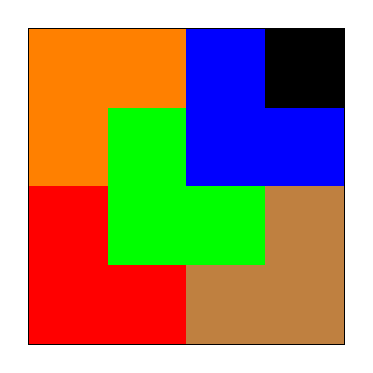
\begin{tikzpicture}[scale=1]
        \draw[step=1cm,gray,very thin] (0,0) grid (4,4);
        \draw[thick] (0,0) rectangle (4,4);
        
        % Example tiles (you can modify or add more as needed)
        \fill[orange,opacity=1] (0,2) rectangle (2,4);
        \fill[brown,opacity=1] (2,0) rectangle (4,2);
        \fill[red,opacity=1] (0,0) rectangle (2,2);
        \fill[green,opacity=1] (1,1) rectangle (3,3);
        \fill[blue,opacity=1] (2,2) rectangle (4,4);
        \fill[black,opacity=1] (3,3) rectangle (4,4);
        % \fill[green,opacity=0.5] (4,3) rectangle (5,5);
        
    \end{tikzpicture}
    \caption{Example of a 4x4 grid with some tiles}
\end{figure}

\subsubsection{Base case}

\begin{align*}
    \text{Base case is } 2^{1}
\end{align*}

wich is just a 2 by 2 grid. only 4 ways to tile it with L shape tiles.

\subsubsection{Recursive case}

$ 2^2 $ comes next. We can divide the grid into 4 quadrants. We can tile the grid by tiling the 4 quadrants.

Did quicksort runthrough.


\end{document}